\documentclass{article}
\usepackage{amsmath}
\usepackage{amsthm}
\usepackage{amssymb}
\usepackage{ctex}
\usepackage{enumerate}
\usepackage{hyperref}
%\usepackage{draftwatermark}
\usepackage{titlesec,titletoc}
\usepackage{cases}
\usepackage{tikz}
\usepackage{pdfpages}
\usepackage[abs]{overpic} 
% define the plot style and the axis style
\tikzset{elegant/.style={smooth,thick,samples=50,cyan}}
\tikzset{eaxis/.style={->,>=stealth}}

\newtheorem{example}{例}[section]             
\newtheorem{theorem}[example]{定理}
\newtheorem{definition}[example]{定义}
\newtheorem{axiom}[example]{公理}
\newtheorem{property}[example]{性质}
\newtheorem{proposition}[example]{命题}
\newtheorem{lemma}[example]{引理}
\newtheorem{corollary}[example]{推论}
\newtheorem{remark}[example]{注}
\newtheorem{condition}[example]{条件}
\newtheorem{conclusion}[example]{结论}
\newtheorem{assumption}[example]{假设}

\renewcommand\contentsname{\centering 目录}


\begin{document}
	\thispagestyle{empty}
	\begin{overpic}[abs, scale=0.5]{blank.png}
		\put(340,60){
\includegraphics[scale=2.5]{logo.png}}
		\put(350,-350){
\includegraphics[scale=2.5]{ahu.png}}
		%\put(350,-350){\includegraphics[scale=5]{ele.png}}
	\end{overpic}
	\put(-10, -150){\zihao{1} \bf《高等数学(一)》辅导资料}
	\put(83,-235){\zihao{4} \bf \today 编译}
	\newpage
	\thispagestyle{empty}
	\mbox{}
	
	\newpage
	\tableofcontents
	
	\newpage
	\thispagestyle{empty}
	\mbox{}
	
	\newpage
	\phantomsection
	\addcontentsline{toc}{section}{前~言}
	\begin{center}
		\zihao{3}
		前~~言
	\end{center}

	当我知道在一个我不存在于其中的QQ群里分享着班级同学们自做的手写答案的时候,我是震惊的。一来,我以为这样的东西之前就会有人制作,就算不完善,至少覆盖了大多数题目。毕竟总会有作业,只要把作业拍照做成文件即可,难度不大。二来,班上的班委(电子班和电类一班班长及团支书商定)主动组织了这样的事情。再有就是,这帮小崽子竟然瞒着我。
	
	多多少少地,我受到了一些触动,觉得既然手写稿都有了,用图像识别工具转换成\LaTeX 命令做成规整的电子版想必更好。而且遇到疫情,大一考试得等到下学期回来再考,有足够的时间。
	
	事实证明我的想法有些欠考虑,两百多页的手写稿,有些同学的笔迹识别率稍高,有些同学的笔迹则几乎无法识别,平均下来一页手稿要半小时甚至一小时才能完成,自己一点一点折腾肯定来不及了。只得向各位同学求助,有愿意帮忙的同学可以用Word写好汇总到曾繁博那里。
	
	开始时电子班有几位同学主动参与Word文档的编写工作,之后,在手写PDF答案制作完成后,先前电子三个班制作手写PDF答案的同学也都克服各种困难,加入了Word文档的编写工作中,使得进度大大加快。
	
	在这里记下所有参与到这个过程的同学姓名,他们是电子信息工程学院2021级电子一、二、三班和电类一班的:
	曹翔,陈磊,陈丽缘,邓黎婷,狄康,丁雨暄,丁兆强,董文凝,桂成达,黄勃铭,黄涛,江琦,金泽平,琚晗平,李帆,廖浩天,刘浩宇,刘奕阳,陆康超,马少轩,欧阳璇,祁家乐,饶家洛,苏国泰,孙浩,汪国锋,汪骏杰,汪天琪,王点点,王开,魏子昂,吴华东,项丙才,谢梦园,谢婷婷,许家栋,杨佳儒,于点,曾繁博,张圣强,张嗣杰,张伟涛,张祥哲,章子楚,钟仕杰,周方元,周幼洋,朱立扬。
	
	这样一份资料的出现,必然会有正反两方面的影响,最直接的一定是方便了这次及以后同学们的复习。但是另一方面,它也会为将来想要抄作业的同学大开方便之门。不过我觉得,手写稿答案的完成已经让那些想要抄作业的同学如愿以偿,是否美观并不会影响他们抄或者不抄。所以,这份资料的出现一定是利大于弊的。
	
	下面是关于本资料的一点说明:
	
	\begin{itemize}
		\item 这份资料做起来十分辛苦,里面也无法避免地有一些纰漏,请各位同学使用时多多理解和包涵,如遇不周全的地方,请辩证看待。
		\item 如前所述,参考本资料时请多多思考资料中的解法是否合理正确。如果有问题,为什么这么做不可以,自己能不能有正确的方法。
		\item 大学里自己要对自己负责,如果有同学决定用这份参考资料来应付高数作业,请想想清楚上大学是为了什么。
	\end{itemize}
	
	再次感谢所有参与了制作这份资料的同学,你们的付出不仅方便了同届的同学,更使得后来的学弟学妹们拥有了一份属于安大学子自己的复习资料!
	
	最后,祝各位同学高数考试顺利;在安徽大学寻得将来能够对抗各种负面情绪的珍贵回忆。
	
	\vskip 3cm
	\hfill 翡翠湖大叔
	
	\hfill 2022.1.26
	
	
	
	\newpage
	\phantomsection
	\addcontentsline{toc}{section}{第2章}
	\mbox{}
	\vspace{4cm}
	\begin{center}
		\zihao{1}
		第2章
	\end{center}
	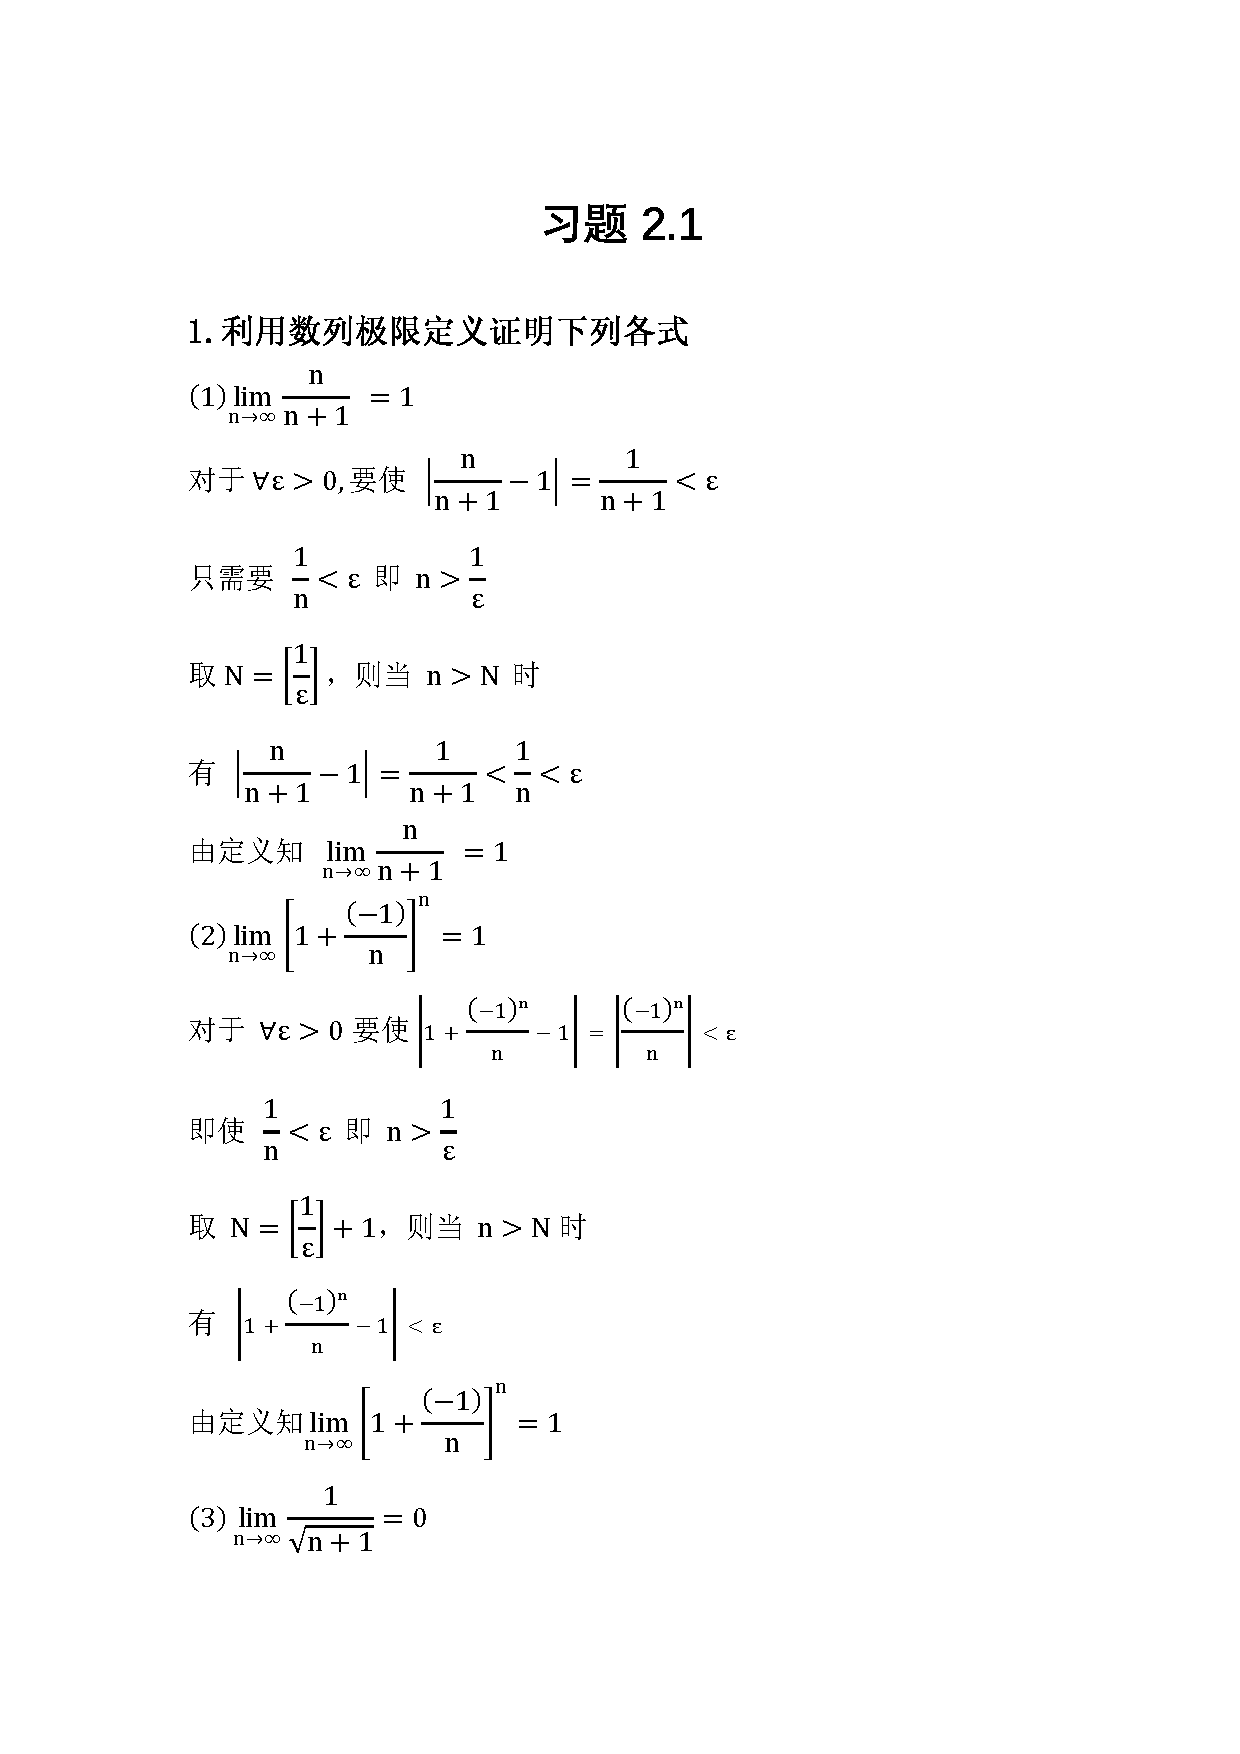
\includepdf[pages=-]{./chapter2.pdf}
	
	\newpage
	\phantomsection
	\addcontentsline{toc}{section}{第3章}
	\mbox{}
	\vspace{4cm}
	\begin{center}
		\zihao{1}
		第3章
	\end{center}
	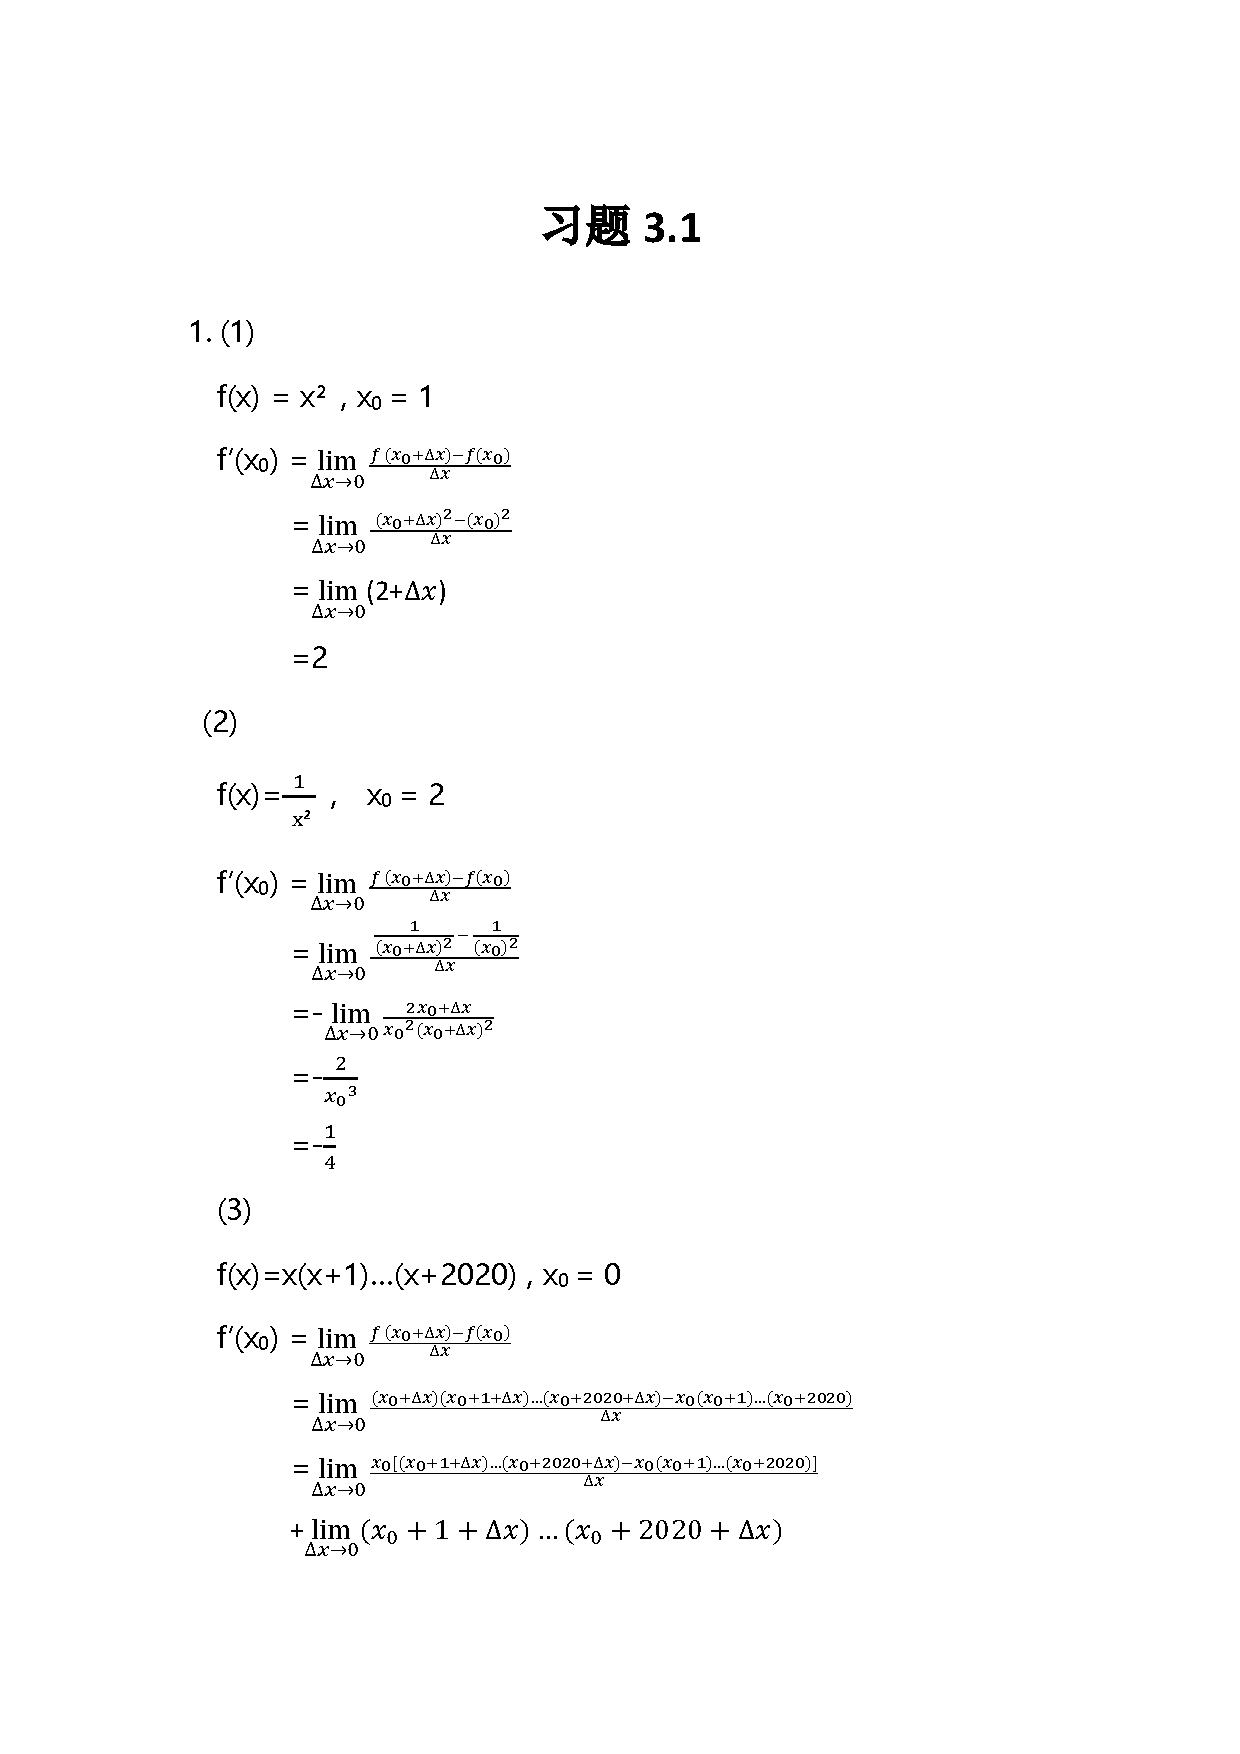
\includepdf[pages=-]{./chapter3.pdf}
	
	\newpage
	\phantomsection
	\addcontentsline{toc}{section}{第4章}
	\mbox{}
	\vspace{4cm}
	\begin{center}
		\zihao{1}
		第4章
	\end{center}
	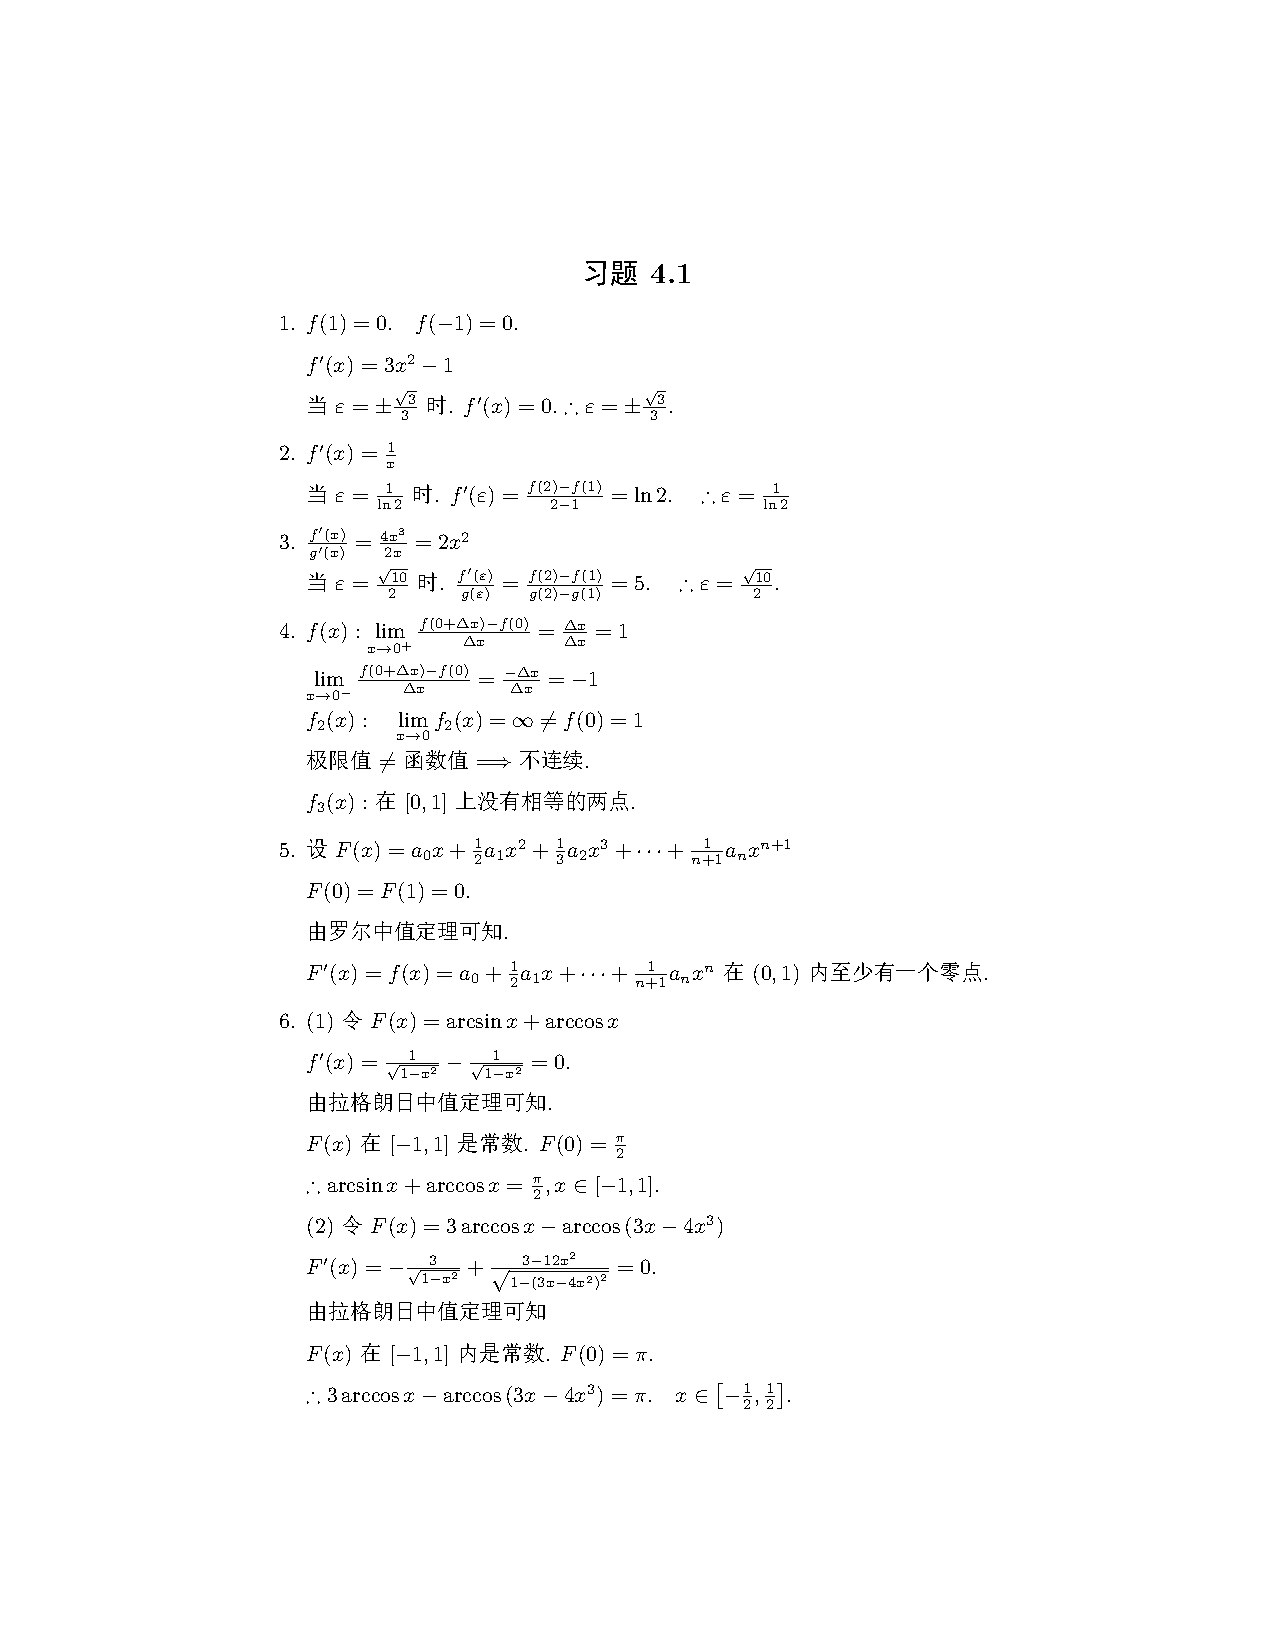
\includepdf[pages=-]{./chapter4.pdf}
	
	\newpage
	\phantomsection
	\addcontentsline{toc}{section}{第5章}
	\mbox{}
	\vspace{4cm}
	\begin{center}
		\zihao{1}
		第5章
	\end{center}
	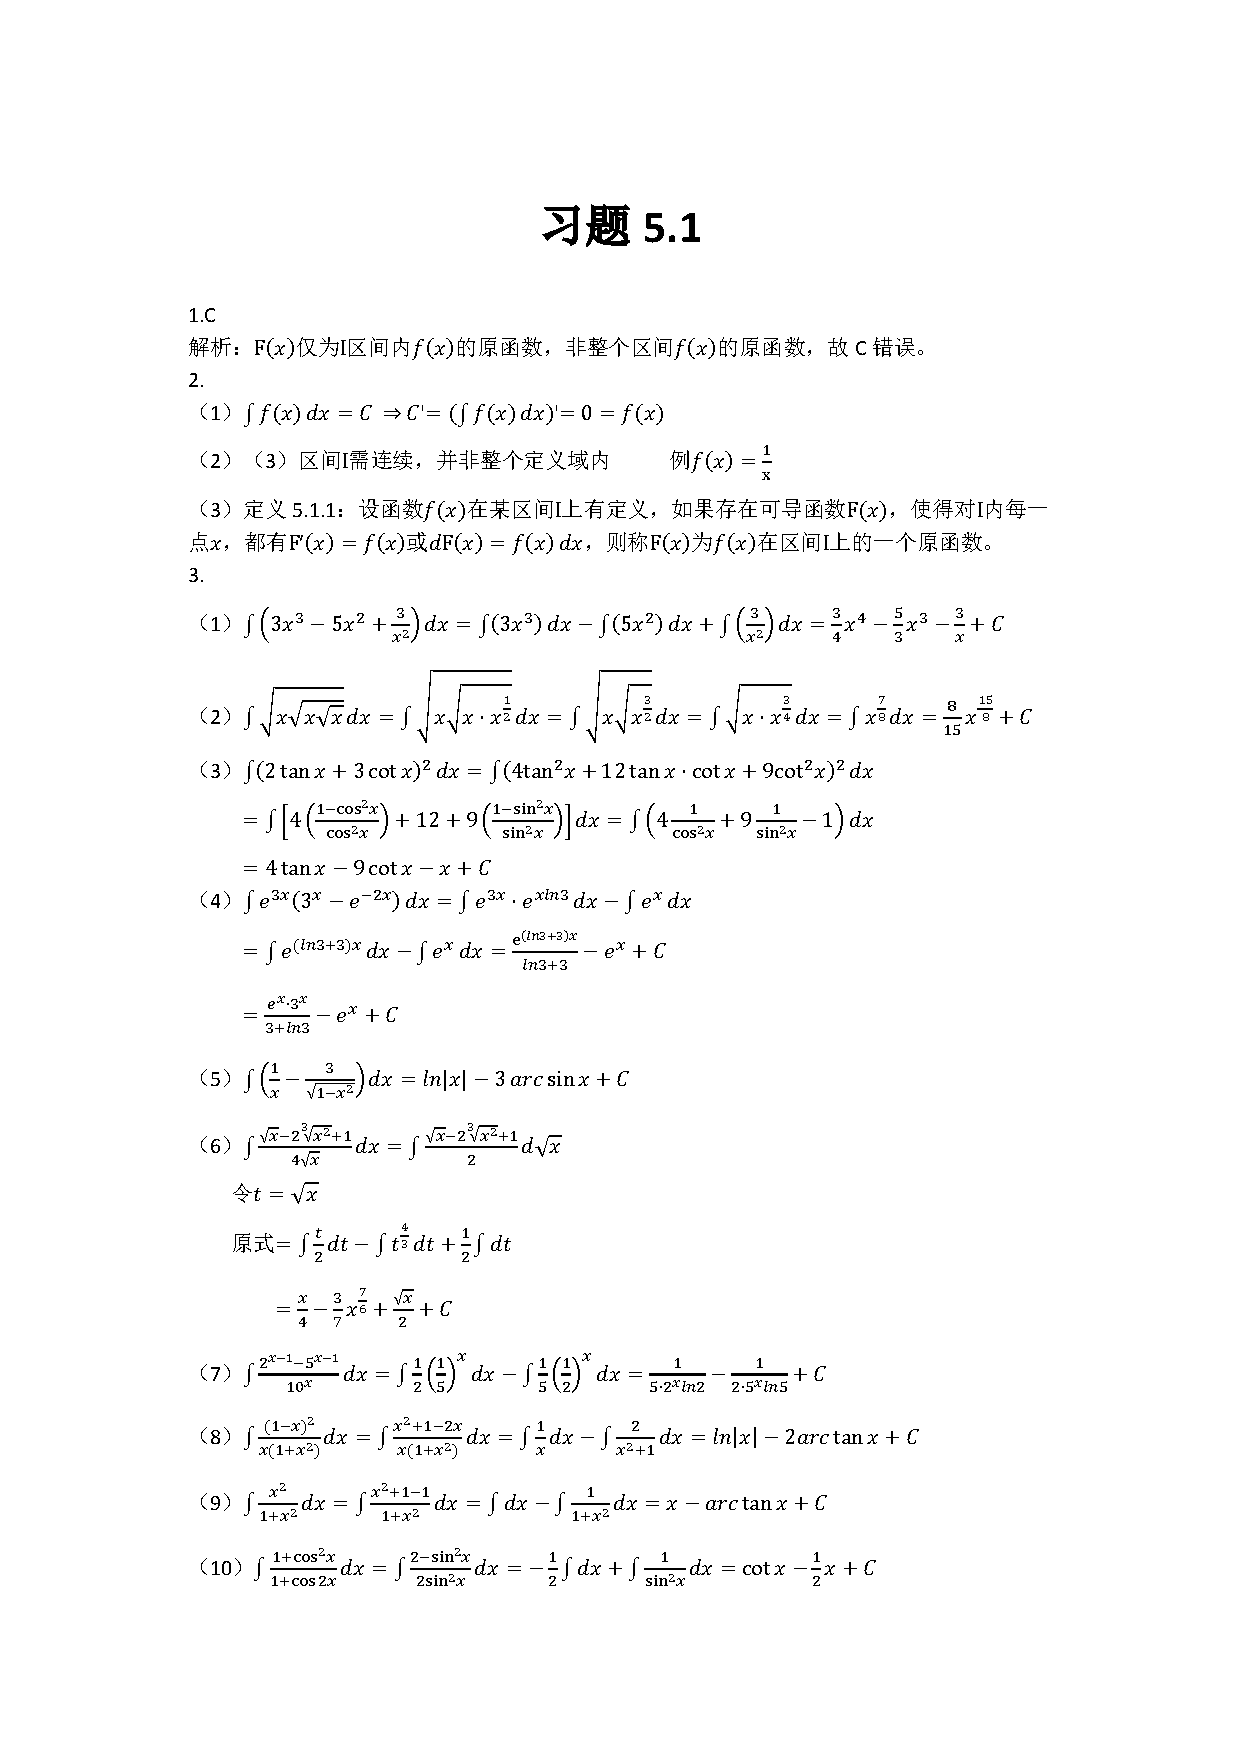
\includepdf[pages=-]{./chapter5.pdf}
	
	\newpage
	\phantomsection
	\addcontentsline{toc}{section}{第6章}
	\mbox{}
	\vspace{4cm}
	\begin{center}
		\zihao{1}
		第6章
	\end{center}
	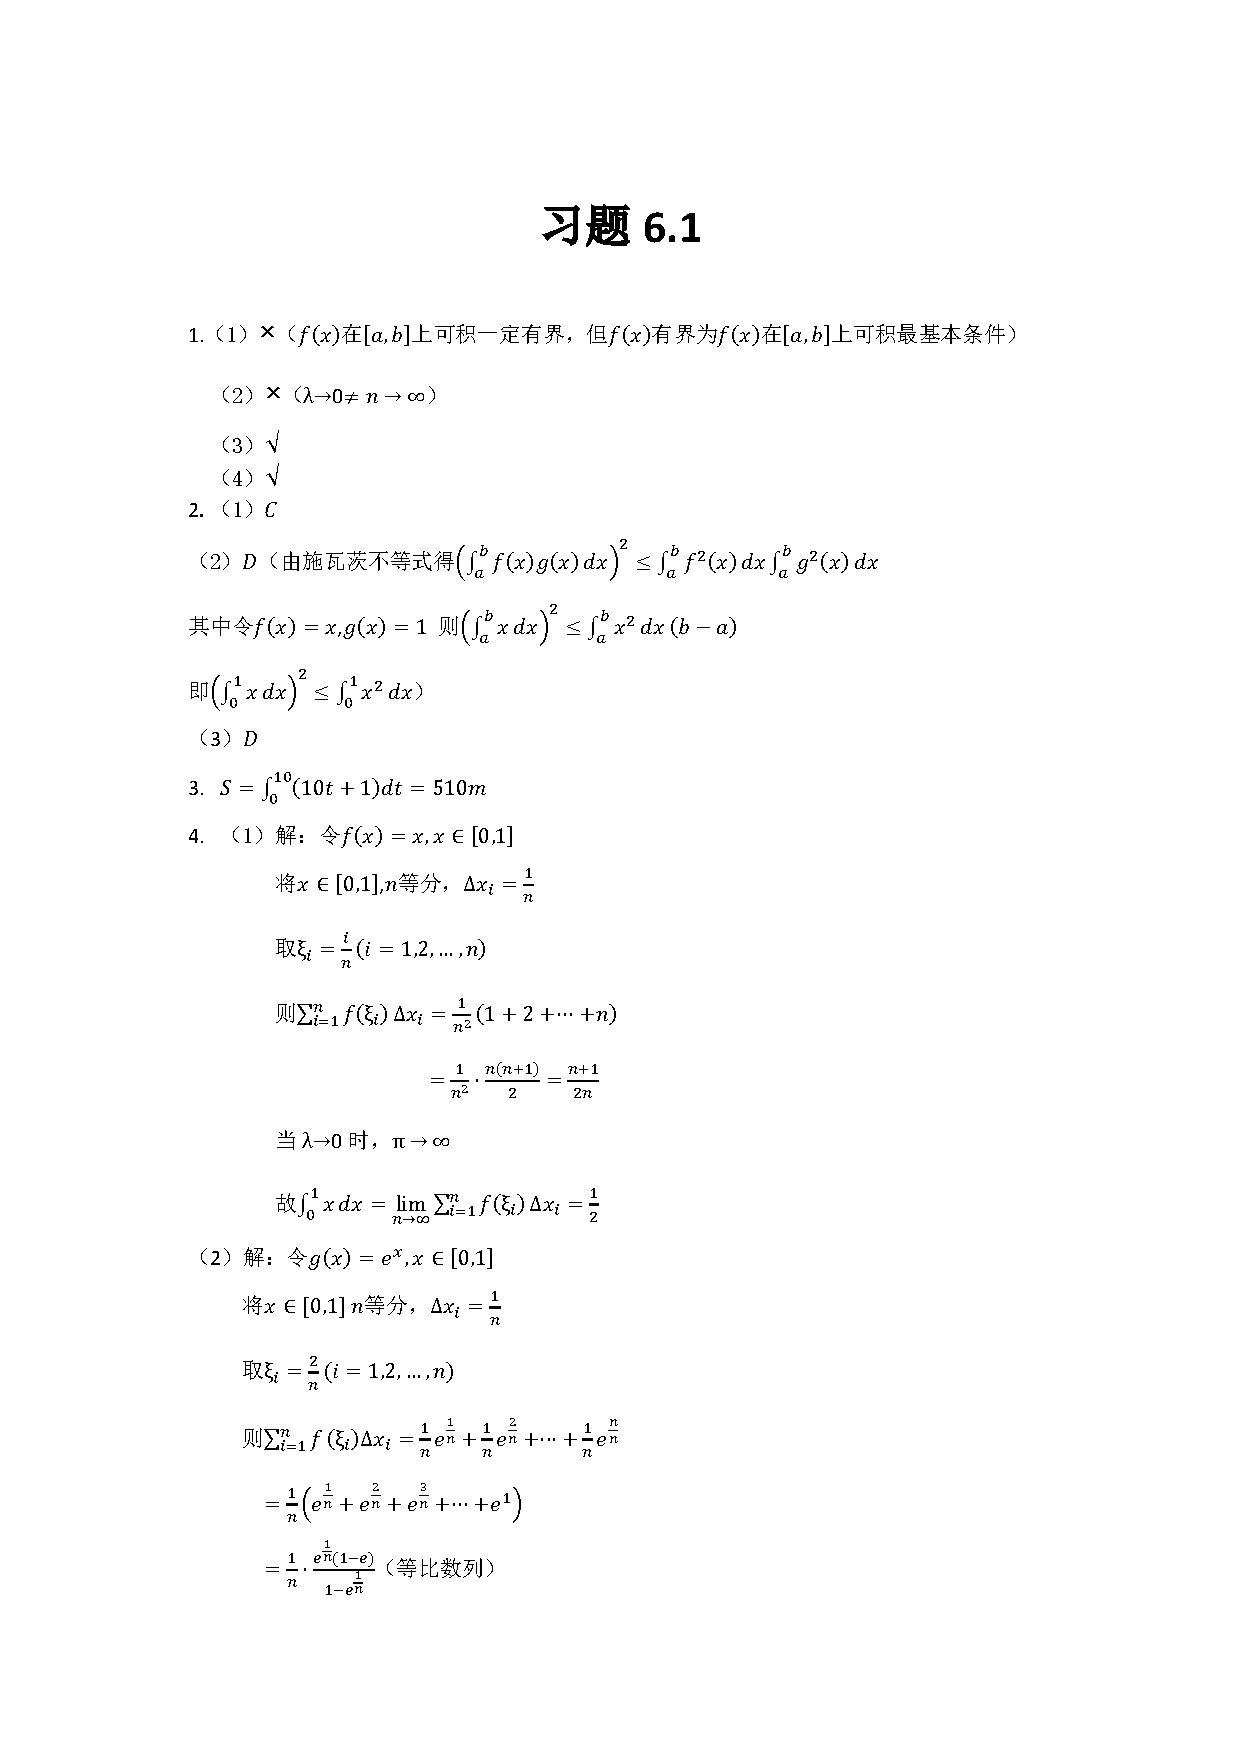
\includepdf[pages=-]{./chapter6.pdf}
	
	\newpage
	\phantomsection
	\addcontentsline{toc}{section}{第7章}
	\mbox{}
	\vspace{4cm}
	\begin{center}
		\zihao{1}
		第7章
	\end{center}
	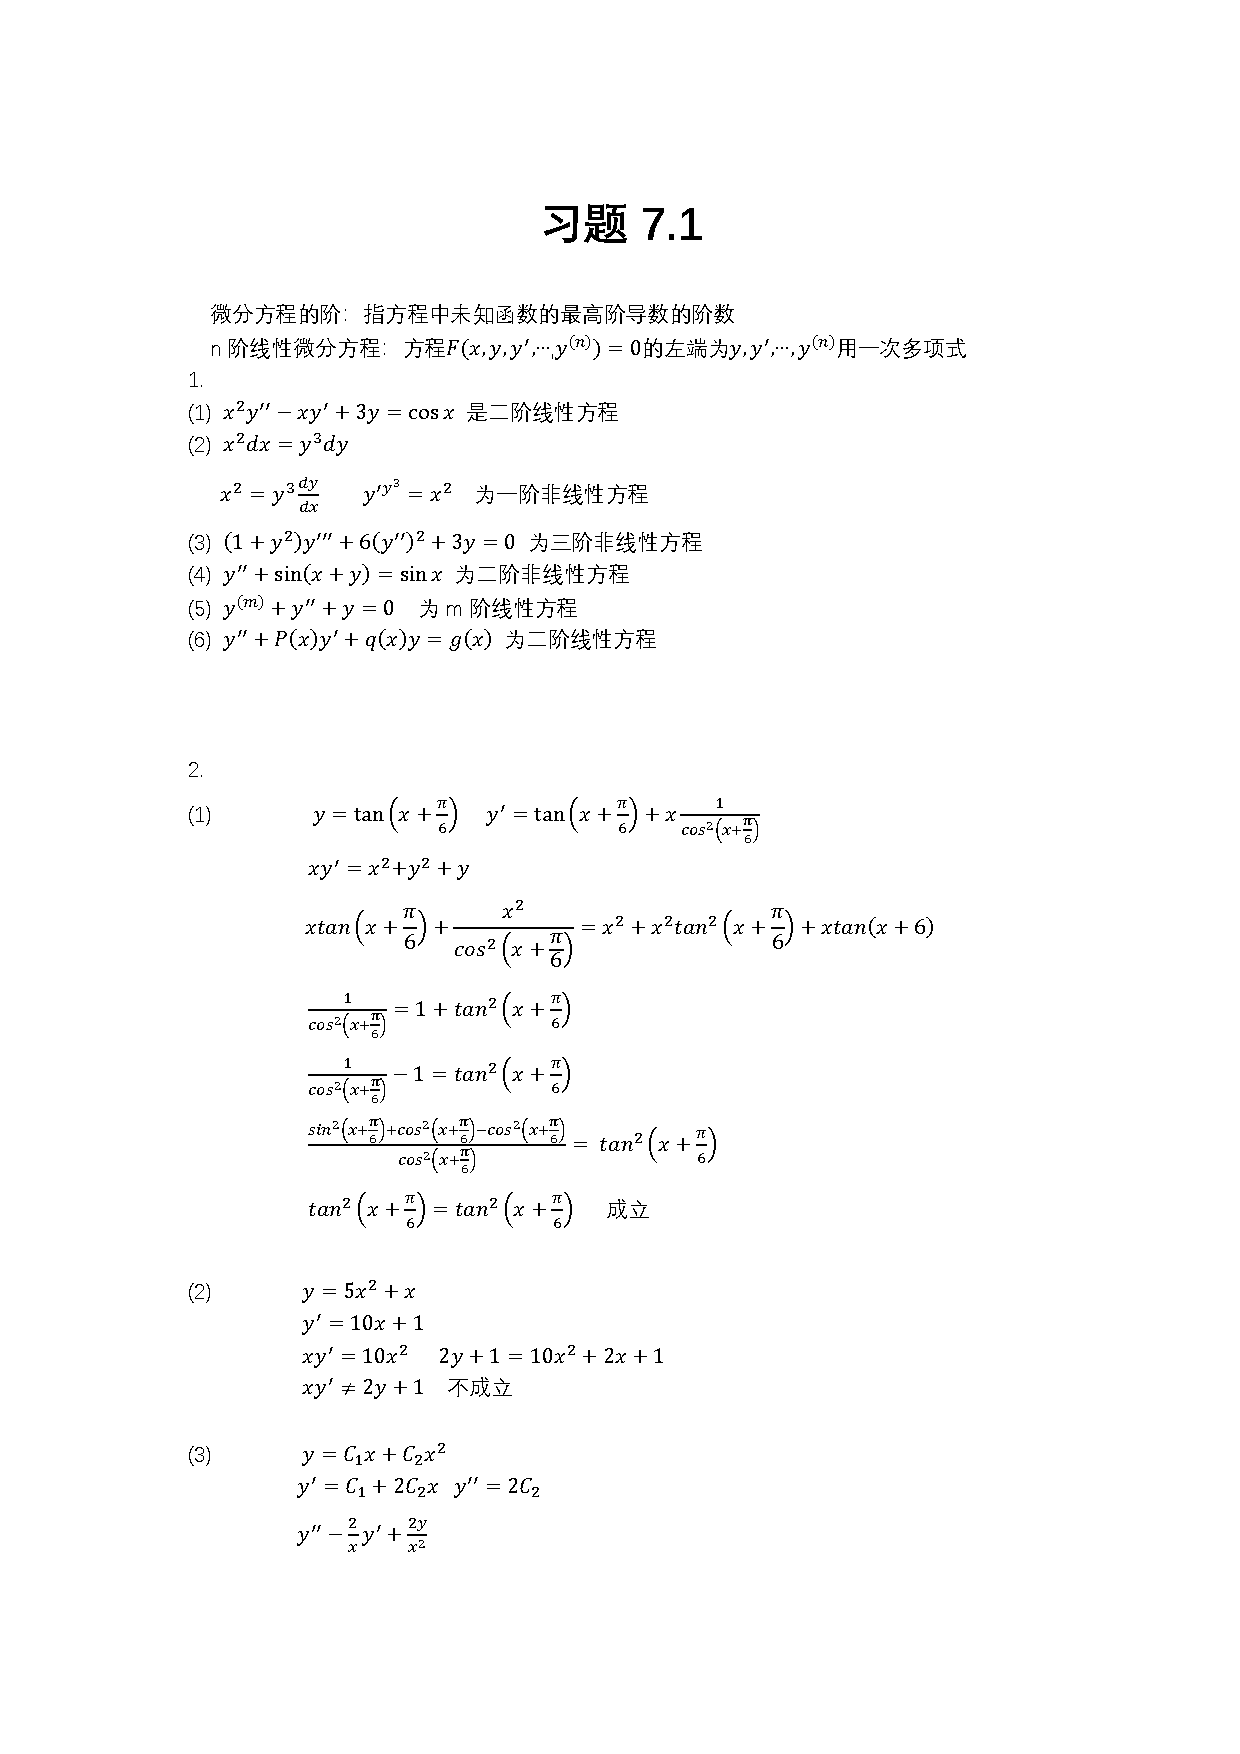
\includepdf[pages=-]{./chapter7.pdf}
\end{document}
